%
\documentclass[runningheads]{llncs}
%
\usepackage{makeidx}  % allows for indexgeneration
\usepackage{amsmath} % allows for \text{}
\usepackage{graphicx}
\usepackage{float}
%
\begin{document}
%
%\frontmatter          % for the preliminaries
%
%\pagestyle{headings}  % switches on printing of running heads
%
%
%\mainmatter              % start of the contributions
%
\title{Online Outlier Detection over Large Datasets}
\titlerunning{Online Outlier Detection}  % abbreviated title (for running head)
\subtitle{Seminar - Multimedia Retrieval and Data Mining}
%
\author{Matthias Hansen}
\authorrunning{Hansen} % abbreviated author list (for running head)
%
%
\institute{Data Management and Data Exploration Group\\
RWTH Aachen University\\
Germany\\
\email{matthias.hansen@rwth-aachen.de}}

\maketitle              % typeset the title of the contribution

\begin{abstract}
Performing Distance-Based Outlier Analysis on Large Datasets poses a challenge with respect to computation time. Due to its $n\log(n)$ complexity, the kd-tree based algorithm for $k$-nearest neighbor search is not applicable for interactive outlier exploration over data sets whose exceed several hundred mega- or even several gigabytes. In this paper, we present a system that preprocesses the results of an initial application of the standard algorithm and stores them in memory to efficiently support any following outlier detection queries and also two novel outlier analysis operations that allow data analysts to gain insight into the outlier status of relevant parts of the data set much more quickly than the traditional approach of repeatedly finding $k$-nearest neighbors would.
\end{abstract}
\section{Motivation}
Finding outliers in data is a problem frequently encountered in data analysis. For example credit card providers use outlier detection to find transactions that could be fraudulent. Similarly, in a network security context, outlier detection can be used to identify intruders. It has also been used for goals as diverse as data cleaning, financial planning and severe weather prediction.
%TODO: add citation as proof for the usage

\subsection{Outlier Definitions}

There is no universally accepted precise definition of what constitutes an outlier in a data set\cite{kriegeldefinitions,outlier_definitions}. Instead, several different definitions are used as appropriate for the task at hand.

Traditionally, outliers have been defined with respect to a statistical distribution. In this approach, every data point to which the distribution assigns a probability below some threshold chosen by the analyst is classified as an outlier. However, this is only applicable if those points that are not outliers are known to follow a specific distribution. This is not always the case and choosing a statistical distribution so that it reflects the data set is challenging and may require domain knowledge and--especially for multivariate data--knowledge about statistics.

A competing outlier definition is the distance-based outlier. A point is a distance-based outlier if its $\varepsilon$-neighborhood with respect to some distance measure (typically the euclidean distance) contains less than $k$ points, where $\varepsilon$, $k$ and the distance measure can be chosen as necessary for the task at hand.

\begin{definition}[Distance-Based Outlier]
    Let DB be a set of tuples. A data point $p\in DB$ is an outlier with respect to a parameter setting $(\varepsilon,k)$ if

    $|\{q \in DB | d(p,q) < \varepsilon\}| < k$.

    $O_{(\varepsilon,k)}(DB) := \{p\in DB \;| \;p\;\text{ is a distance-based outlier w.r.t. }(\varepsilon,k) \}$
\end{definition}

This definition is impartial to the distribution of the data and it is especially useful for geospatial data, where the Euclidean distance has additional meaning apart from indicating (dis-)similarity. Drawbacks of this definition include inability to cope with arbitrarily high-dimensional data, since the distances of the most-distant and the least-distant points approach each other as the dimensionality of data set grows--a phenomenon referred to as the \emph{curse of dimensionality}\cite{curse_of_dimensionality}.
\subsection{Computation Methods for Distance-Based Outliers}

The na{\"i}ve way to detect distance-based outliers is to simply compute the distances between each pair of points. From the resulting distance matrix, the k-th closest other point for every point $p_i$ can be found by scanning $p_i$'s row in the distance matrix. Then, one has to check whether the distance to this k-th closest point is bigger than $\varepsilon$. If this is the case, then $p_i$ is an outlier.

The time and space complexities of this algorithm are both in $\mathcal{O}((n\cdot d)^2)$ ($n$ being the number of rows and $d$ the number of columns in the DB), so the algorithm does not scale well for large amounts of data.

Faster algorithms to solve this problem are typically based on spatial index structures. For example, a kd-tree based algorithm exists that solves this problem in $\mathcal{O}(n\cdot d \cdot\log(n\cdot d))$, by first finding the $k$-nearest neighbors of each $p_i$ and then comparing the distance to the $k$-th nearest neighbor to $\varepsilon$ to find out whether $p_i$ is an outlier. 

This algorithm clearly performs better for large datasets. However in our experiments we found that for e.g. a geospatial dataset\footnote{Further information about this dataset and the experiments carried out with it is to be found in the evaluation section} of roughly 600 Mb, a single outlier detection query already takes about 6 minutes on a typical consumer laptop computer. Since the time complexity of the algorithm is (slightly) above linear, datasets that are even 10 times this size will already cause considerable processing times even on faster machines.

One solution to this problem is to use parallelism \cite{parallel_knn}
however parallelizing the $k$nn-queries is typically difficult to implement, requires expensive hardware (especially when parallelizing to many machines) and does not offer more than a linear speedup.

Another possibility is to use the DOLPHIN system\cite{dolphin}, which handles large data sets efficiently. However, this system was proposed in order to handle data sets that do not fit into the memory of the computer by minimizing disk access. For datasets that do fit into memory, this system does not even perform faster than the kd-tree algorithm.

These performance issues are not as grave if only one isolated outlier detection query has to be performed. However, a typical use case for outlier detection is exploratory data analysis, where it is not clear ahead of time whether one set of parameters ($k$,$\varepsilon$) produces the desired outlier detection result. An analyst might, for example, run an outlier detection query with a value of $k$ that is very high, wait a long time for the result, and then find out that the outlier detection algorithm has classified every point as an outlier. They would then have to re-run the outlier detection algorithm with a different set of parameters, completely recomputing the $k$-nearest neighbors in the process. This process might have to be repeated multiple times until a satisfying result is found. In this scenario, the restrictive cost of outlier detections is a big problem.
\subsection{Considerations for a New Outlier Detection System}
As mentioned before, common distance-based outlier algorithms recompute a $k$-nearest neighbors ($k$nn) query on every outlier detection request. However, one $k$nn result can be used repeatedly because querying for e.g. the 5 nearest neighbors also reveals the fourth, third, second etc. nearest neighbor and thus outliers can be detected for any parameter setting $(\varepsilon,k^\prime)$ where $k^\prime \leq k$ in linear time simply by storing the knn result.

If it is known ahead of time that certain parameter combinations are not of interest, then parts of the knn result can be discarded while still allowing for this linear-time outlier detection. For instance, if it is known that outlier detection queries with $k < 3$ are not ``useful'' for a dataset, then all information about first and second nearest neighbors can be deleted. Similarly, if maximum and minimum ``useful'' values for $\varepsilon$ are known then all points whose closest neighbor is above the maximum $\varepsilon$ are clearly already outliers for any ``useful'' parameter setting. Nearest neighbor information on these points can thus also be discarded and they can be regarded \emph{const outliers} with respect to the ``useful'' parameter settings. The same procedure can be applied where even the distance of the k-th nearest neighbor is above the minimum useful value for $\varepsilon$ and these values can be classified as \emph{const inliers}. If many points are either \emph{const inliers} or \emph{const outliers}, then outlier detection has to merely consider the remaining points, the \emph{outlier candidates}, greatly decreasing both memory usage and processing time. Under the assumption that outliers are the minority of points in the data set and if the range of ``useful'' values for $k$ and $\varepsilon$ is chosen carefully, this means that the amount of data that has to be stored in memory to allow for this linear-time outlier detection is not much larger than the size of the original data set.

Additionally, the traditional outlier detection query is not the only conceivable mode of gaining information about outliers from a data set. We propose two other interesting problems that a new outlier detection should be able to solve:

\begin{definition}[Comparative Outlier Analytics (CO)]

\noindent Given $P\subseteq DB$, find maximal $Q\subseteq DB$, such that the following proposition holds:

\noindent $\forall (\varepsilon,k) P \subseteq O_{(\varepsilon, k)}(DB) \implies \forall (\varepsilon,k)Q\subseteq O_{(\varepsilon, k)}(DB)$
\end{definition}

\begin{definition}[Outlier-Specific Parameter Space Exploration (PSE)]

\noindent Given $P\subseteq DB$ and $\delta \in (-1,1)$, identify all parameter settings $(k,\varepsilon)$, such that

\noindent(1) $|O_{(k,\varepsilon)}(DB)| = (1 - \delta) \cdot |P|$

\noindent(2) $O_{(k,\varepsilon)}(DB) \subseteq P$ if $\delta \geq 0$ or $P \subseteq O_{(k,\varepsilon)}(DB)$ if $\delta \leq 0$
\end{definition}

Algorithms to solve these problems would allow analysts to use knowledge about the outlier status of certain points in order to find outliers without relying too much on the abstract notion of \emph{parameters}. For instance, in the credit card fraud detection scenario, it could be known to them that certain transactions were fraudulent and these transactions could then be used in a CO query to find other transactions that might be fraudulent.

Similarly, the analyst might also know from a statistic maintained by their business that a certain percentage of transactions is fraudulent. They could apply PSE to a set of known fraudulent transactions and set delta such that the returned parameter settings produce outlier sets with a size of that percentage compared to the data set.

To conclude, a new outlier detection system should take ranges instead of fixed values for $\varepsilon$ and $k$ and use these to support efficient outlier detection queries within these ranges as well as the other outlier operations we presented.
\section{Overview of the ONION System}
The ONION system\cite{onion} addresses the considerations of the previous section by having the user provide a parameter set $(k_{min},k_{max},\varepsilon_{min},\varepsilon_{max})$ instead of single values for $k$ and $\varepsilon$ and splitting the Outlier Analysis task into an offline and an online phase.

In the offline phase, an initial knn query is performed and the result is processed into a series of three data structures: \emph{O-Space}, \emph{P-Space} and \emph{D-Space}, each of them allowing for more efficient answering of some of the three types of queries explained in the previous chapters.

In the online phase, Outlier Detection, Comparative Outlier Analytics and Outlier-Centric Parameter Space Exploration queries can be issued by the user. These queries can be processed by consulting the data structures computed in the offline phase without referring to the original data set.

The ONION system takes its name from this \underline{on}line outlier detect\underline{ion} approach.

\section{Offline Phase}

The offline phase consists of the creation of three data structures in order:

\begin{itemize}
 \item O-Space (ONION Space) is a data structure obtained by carrying out a $k$nn search and then saving the results, discarding unnecessary information.
 \item P-Space (Parameter Space) is created by sorting the knn results by the computed distance value for each value of k. This results in an ordered list of valuees to which binary-search style algorithms can be applied for more efficient outlier detection.
 \item D-Space (Domination Space) is based on a \emph{domination} relation, in which one point is said to dominate another if every parameter setting that marks it as an outlier also marks the other as an outlier. This relation typically holds among most data points and information about this relation can be encoded within a set of ordered lists (or alternatively a forest of search-trees).
\end{itemize}

It is important to note that not the entire offline phase has to be performed to allow for use of the ONION system. Most of the three outlier analysis operations can be carried out using any one of these data structures, however the more of this preprocessing is performed, the faster subsequent outlier queries can be performed. Depending on the data set and parameter values, the creation of \emph{O-Space} might e.g. take much longer than e.g. \emph{D-Space}, in which case it might be advisable to carry out the whole offline phase. In other cases the computation of \emph{D-Space} is going to be entirely uneconomical.

As our results in the following chapters will show, \emph{P-Space} construction takes negligible amounts of time and should almost always be carried out, while \emph{D-Space} construction is prohibitively expensive if many outlier candidates have been found.

\subsection{O-Space}
O-Space is computed by carrying out a modified knn query with the parameter $k_{max}$. Specifically  the knn search for each point $p_i$ is modified by aborting once $k_{max}$ points whose distance to $p_i$ is smaller than $\varepsilon_{min}$ have been found because once this condition is known to hold, it is clear that $p_i$ will always be an inlier under any single parameter setting $(k,\varepsilon), \text{ where } k_{min}\leq k \leq k_{max},\; \varepsilon_{min}\leq \varepsilon \leq \varepsilon_{max}$. Under the assumption that most points will be such \emph{const inliers}, this modification reduces the running time of the $k$nn search by a large amount. Apart from this optimization, any $k$nn algorithm can be used, even e.g. parallel or approximate ones.

Similarly, once the $k$nn search has finished, all $p_i$ whose distance to their $k_{min}$-th nearest neighbor is larger than $\varepsilon_{max}$ can be labeled as \emph{const outliers}.

The remaining points are labeled \emph{outlier candidates} and only for these do the $k$nn-query results play any further role.  However, the distances to the $[1,k_{min}-1]$-th nearest neighbors for each outlier candidate can still be discarded. We denote the set of outlier candidates by $OC$.

An example is given to illustrate this:
%TODO: Add example here
The complexity of this \emph{O-Space} construction is dominated by the time needed to compute the knn and therefore depends on the algorithm used for knn search (ideally one that can be performed in $n \cdot log(n)$ time), since all other operations needed to construct \emph{O-Space} can be carried out in linear time.
%TODO: Add example
\subsection{P-Space}
\emph{P-Space} can be computed from O-Space by sorting the distances in each column of the \emph{O-Space} table in ascending order, to allow for binary-search-like processing, reducing the runtime of some of the outlier analysis operations from linear to logarithmic time. Using any efficient sorting algorithm, this can be done in $k \cdot |OC| \cdot log(|OC|)$ time. 

In order to still be able to identify which distance belongs to which outlier candidate after sorting, the index of the outlier candidate has to be carried along into each cell of the table. This tuple of $\text{index},\varepsilon)$ is referred to as a P-Node in the original paper\cite{onion} describing the ONION system.

We provide an example based on the example \emph{O-Space} computation from the previous section:
%TODO: Add example
\subsection{D-Space}
\emph{P-Space}, supports OD queries efficiently. However, CO can still not be computed easily based just on the \emph{P-Space} data structure. This is because outlier detection requires checking for each value of $k \in [k_{min},k_{max}]$ whether a particular point $p_i$ is an outlier if another point $p_j$ is an outlier. We introduce some terminology to tackle this problem:
\begin{definition}[k-domination]
Let $p_i,q_j \in OC;\; k\in [k_{min},k_{max}]$. We say that $p_i$ $k$-dominates $p_j$, $p_j \leq_{k} p_i$ iff. $\forall\varepsilon(p_i \in OD_{(k,\varepsilon)} \implies p_j \in OD_{(k,\varepsilon)})$
\end{definition}
\begin{definition}[(full) domination]
Let $p_i,q_j \in OC$. We say that $p_i$ (fully) dominates $p_j$, $p_j \leq p_i$ iff. $\forall k\in [k_{min},k_{max}](p_j \leq_k p_i)$
\end{definition}
This k-domination relation is clearly transitive, since it essentially just relies on comparing numbers. By extension, the full domination relation is also transitive. However, while k-domination is total, i.e. each point k-dominates or is k-dominated by every other point, the same is not true for full domination. To examine this further, we utilize the graph of this relation.
\begin{definition}[Domination Graph]
The domination graph is the undirected graph created by the domination relation. Each outlier candidate is represented in the Domination graph as a node. Two nodes representing points $p_i$ and $p_j$ are connected by an edge iff. $p_i \leq p_j \vee p_j \leq p_i$.
\end{definition}

Since the domination relation is transitive and represented symmetrically in the graph, any set of outlier candidates among which the domination relation is total forms a subgraph, which is \emph{complete}, i.e. every pair of nodes is connected. To simplify CO, it would be useful to split the domination graph into a maximal set of complete subgraphs and order the points belonging to each subgraph w.r.t. the domination relationship. This could allow for logarithmic complexity comparative outlier analysis. However, the detection of maximal complete subgraphs (so called \emph{cliques}) is a known NP-complete problem. For this reason, this part of the preprocessing can only be performed in acceptable amounts of time if the number of outlier candidates is relatively small. If this is the case, then any algorithm to solve the cliques problem can be used.

Once each \emph{clique} has been found, their nodes can in such a way that they are ordered by domination, thus making outliers binary-searchable w.r.t. domination. The list of these sorted \emph{domination lists} then forms \emph{D-Space}. Our experiments in the later chapter show that these lists sometimes intersects and the number of \emph{domination lists} is usually very small, somewhere between 2 and 6 for all the datasets that we have tested.

We have deviated slightly from the original paper presenting the ONION system\cite{onion} in our description of \emph{D-Space}, by formulating the problem of finding the parts of the relation that are complete in terms of CLIQUES. In the original paper, they used the edge-inverted undirected graph of the domination relation and formulated the solution in terms of another, less well-known NP complete problem called MINIMUM-VERTEX-COVER. In fact, inverting the edges of the domination graph (i.e. constructing for a given graph (E,V) a new graph ($E'$,V), so that $\forall v_1,v_2\in V(E(v_1,v_2) \iff \neg E'(v_1,v_2))$) is the canonical\cite{cormen} reduction from MINIMUM-VERTEX-COVER to CLIQUES and vice versa.

We chose CLIQUES to formulate the problem because it is arguable more well-known  and ``fits'' our intuition better, but also because no software to solve MINIMUM-VERTEX-COVER problem was available to us.

Additionally, the original paper structures the domination lists as trees. However, it is not motivated why trees are a better choice than sorted arrays (which we reffered to as lists here).

\section{Online Phase}
\subsection{Outlier Detection}

Outlier detection can be carried out with the \emph{O-Space} data structure by checking all entries for the selected value of $k$. If their distance is above the selected value for $\varepsilon$, the the respective point is an outlier. Since only Outlier Candidates have to be checked, the time complexity of this algorithm is in $\mathcal{O}(|OC|)$, where the set $OC$ might be only slightly smaller or several orders of magnitude smaller than the original DB, depending on the ranges for $k$ and $\varepsilon$.

Using \emph{P-Space} allows for the use of binary search instead of a scan over the data. Since the distance values are sorted, the search can begin in the middle of the list of distances and then be continued in such a way that the first element that is an outlier will be found. All elements after this one are then confirmed to be outliers. This algorithm's complexity is then in $\log(|OC|)$, which should be quite sufficient even for very large datasets.

Using \emph{D-Space} for this task is actually slightly worse: The sorted domination lists which \emph{D-Space} is composed of have to be searched in a similar algorithm as \emph{P-Space}, so the complexity is logarithmic, but the algorithm has to be applied on each individual list. Let $n_1 \ldots n_j$ be the lengths of the lists, then this algorithm is in $\mathcal{O}(\log(n_1) + \ldots + \log(n_j)) = \mathcal{O}(\log(n_1 \cdot \ldots \cdot \log(n_j))$. Since $|OC|$ is the sum of the lengths of the lists, this is slower than the \emph{P-Space}-based algorithm described above. Additionally, if the $k$nn-distances of each outlier candidate are not saved in the domination lists, it is necessary to ``look them up'' in the \emph{O-Space} data structure, so access to \emph{O-Space} is also needed to support this operation with \emph{D-Space}.
\subsection{Comparative Outlier Analytics}

To find the set of comparative outliers $Q$ for one set of input points $P$, using only the \emph{O-Space} data structure, the entries of the table for each $k$ have to be scanned to obtain the distance values for each point $p_i\in P$ and then all points in that row whose distance is larger than that for the $p_i$ with the largest distance have to be saved. After these sets have been computed for each $k$, their intersection has to be determined. This intersection is the set Q that forms the result. Since the entire table has to be scanned, the time complexity of this algorithm is in $\mathcal{O}(k\cdot |OC|)$.

\emph{P-Space} offers a straightforward improvement on this algorithm: since the distances for each $k$ are sorted, the part of the scan that considers each outlier candidate can be done in logarithmic time. Thus, time complexity will be in $\mathcal{O}(k\cdot \log(|OC|))$.

Using \emph{O-Space} further reduces this complexity: Since it contains information about the domination relationship independent of the value of $k$, one only needs to search the domination lists for the weakest outlier in the input set $P$. All points preceding this point are then clearly comparative outliers. Since the domination lists are ordered, this search can be performed in logarithmic time, i.e. $\mathcal{O}(\log(n_1) + \ldots + \log(n_j))$, where $n_1, \ldots , n_j$ are the lengths of the domination lists as above.
\subsection{Outlier-Centric Parameter Space Exploration}
 
For $\delta=0$, Outlier-Centric Parameter Space Exploration using \emph{O-Space} can be supported by finding the weakest outlier, i.e. the one that needs the lowest value of $\varepsilon$ to become an inlier, for each $k \in [k_{min},k_{max}]$. The time complexity of this is in $\mathcal{O}(|P| * |[k_{min}, k_{max}]|$, which is simply the summed-up cost of finding the weakest outlier for each $k$. In cases where $\delta \neq 0$, answering PSE with \emph{O-Space} requires sorting each individual row of \emph{O-Space}, which is already exactly the same as computing \emph{P-Space}.

Answering PSE using \emph{P-Space} additionally requires access to \emph{O-Space} because random access to $\varepsilon$ values is needed to find the weakest outlier as above and without random access, the complexity of just this subtask is in $\mathcal{O}(|[k_{min},k_{max}]| \cdot |OC|)$, which is much too large. Having used \emph{O-Space} to determine the weakest outliers for each $k$, one can then use their indices within their \emph{P-Space} rows to calculate which oc should be the new weakest outlier. Since all additional operations only have to be done once for each value of $k$, the time complexity of this is the same as the time complexity of answering PSE using \emph{O-Space}.

To answer PSE using \emph{D-Space}, one has to find the weakest outlier in the intersection of the input set P and each domination list, i.e. the weakest outlier in $P \cap \text{ list}_1, \ldots ,P\cap\text{ list}_j$ . This can be done using \emph{O-Space}. Then, the $\delta$ parameter can be incorporated by applying the simple multiplication one would use when answering this query-type using \emph{P-Space} to each domtree. The final parameters can be obtained using \emph{O-Space} as before. The time complexity of this algorithm is dominated by the cost of intersecting the input set and the outliers in the domination lists, which can be performed in $\mathcal{O}(|OC| + |P|)$ using a hash set data structure. We did not find an algorithm that solves this problem with the $\mathcal{O}(|P| + n)$ (where n is the number of domination lists) complexity that is claimed in the original paper.
\section{Evaluation}

We evaluate our implementation of the ONION system on a real world geospatial dataset.

\subsection{Data Set}
For evaluation we used position data from OpenStreetMap\footnote{available at http://download.geofabrik.de} on the South American continent and some South Pacific islands. This data was obtained by parsing the xml data of the OpenStreetMap project and saving the longitudes and latitudes of all ``nodes'', i.e. all points on the map that represent houses, traffic signs, parking spaces etc. This preprocessing resulted in a data set of roughly 80 million coordinates. The data set was subsequently normalized to facilitate parameter selection. Appropriately sized subsets of this datasets were extracted by random sampling.
\begin{figure}[H]
\caption{A Normalized, Randomly Sampled Subset of the Data Set}
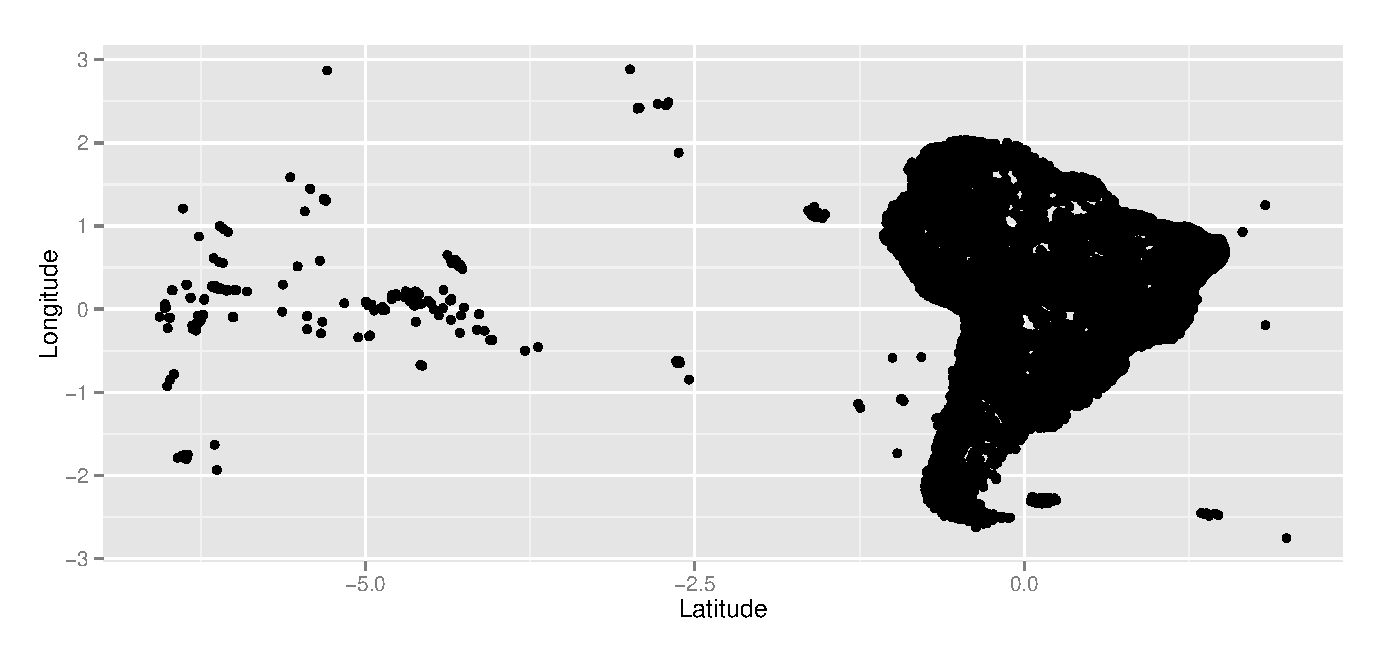
\includegraphics[width=.68\textwidth]{images/south-america-osm.eps}
\end{figure}
\subsection{Environment}
Experiments were carried out on a desktop computer running Mac OS X with a 2.5GHz quad-core processor and 12 GB of RAM. Some of the earlier results in the paper were obtained with a laptop running Ubuntu that had a similar processing power. 

The implementation was done in R, except for the initial $k$nn query and most of the dspace construction, which could mostly be accomplished by using existing R and C++ libraries along with some C++ code that we wrote.
\subsection{Results}
To obtain information about the running time of the ONION system, we ran the offline phase on several subsets of the OpenStreetMap data set with a parameter setting of $([k_{min},k_{max}],[\varepsilon_{min},\varepsilon_{max}] = ([3,6],[0.05,0.1])$
\begin{figure}[h]
\caption{Running Time of $K$nn-query and Subsequent \emph{O-Space} Construction}
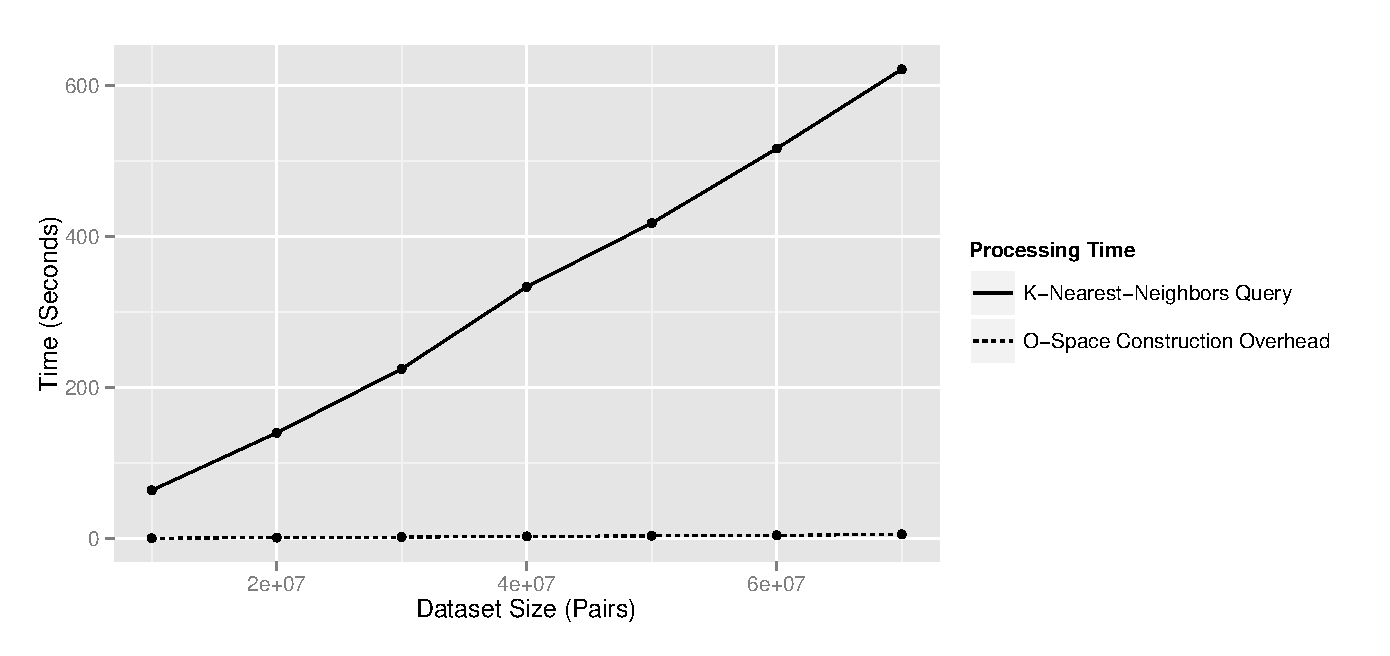
\includegraphics[width=\textwidth]{images/ospace_vs_knn.eps}
\end{figure}

As can be seen here, the $k$nn query has a practically linear running time with respect to the dataset size and the overhead of constructing the \emph{O-Space} data structure is very small in comparison. This raises the question if \emph{O-Space} construction is constant.


\begin{figure}[H]
\caption{Running Time of Data Structure Constructions}
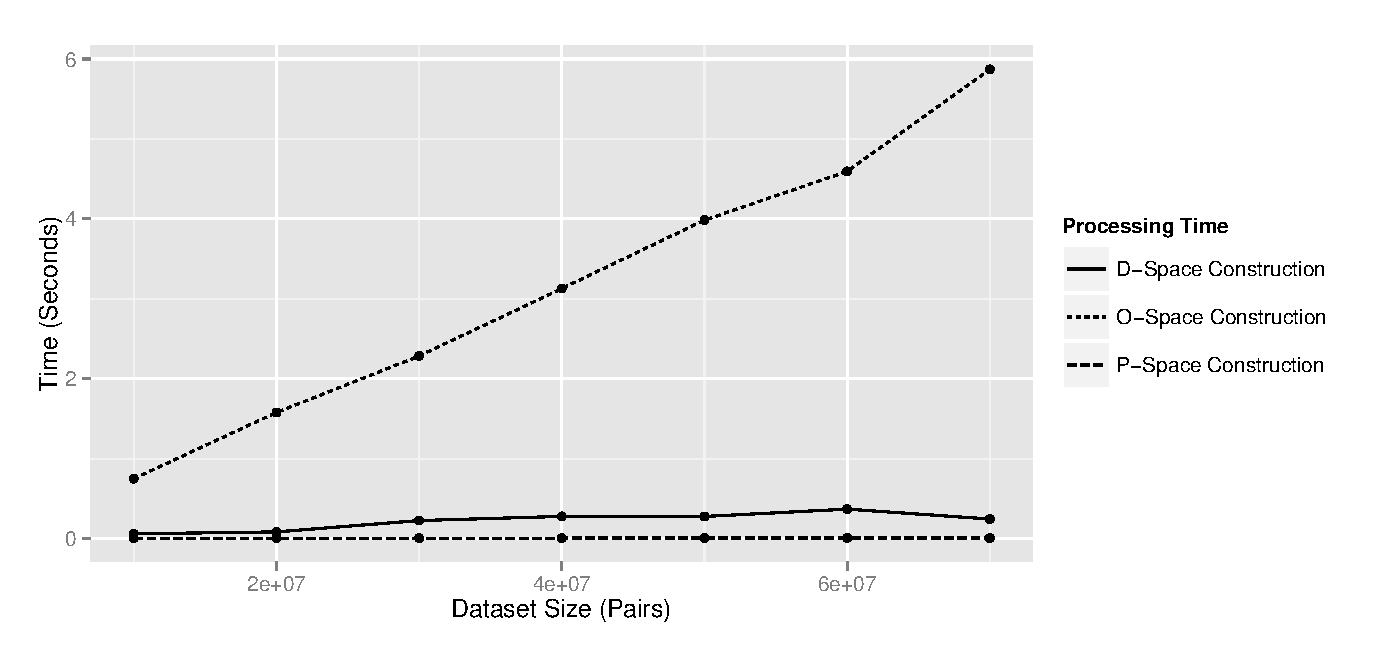
\includegraphics[width=\textwidth]{images/spaces_construction.eps}
\end{figure}

As this figure shows, this is not the case: \emph{O-Space} construction is linear. This is not surprising, since the main operations performed in its construction apart from the $k$nn query are the identification of const outliers and const inliers. Both are performed in one scan over the dataset.
This graph also shows that the construction times of the other data structures do not depend on the number of points in the original dataset. Instead, the number of outlier candidates, which is not monotonous w.r.t. dataset size has to be used as reference. To this end, we performed additional queries with a relatively small(3000000 points) subset of the data and various parameter settings to confirm our suspicions about the running times of \emph{D-Space} and \emph{P-Space}.



\section{Conclusion}
We have established a novel system for outlier detection that facilitates outlier detection and have shown that this system is not much slower than the established $n\cdot \log(N)$ algorithms for the first query and allows for drastically improved processing time on any subsequent outlier detection query by sacrificing memory to store data structures. The size of these data structures is not much larger than the original data set if and only if the parameters are chosen carefully so that $|[k_{min},k_{max}]| \cdot |OC|$ is small. Choosing such a set of parameters in an Exploratory Data Analysis setting may be possible by consulting a visualization of the data but can also sometimes require experimentation, i.e. running the offline phase multiple times. In these cases, many initial queries may fail due to restrictions on the available memory and the performance gains from the ONION system are negated for all but the last few queries in which the parameters are ``fine-tuned''. 

The other outlier analysis operations proposed also suffer from this problem, since they cannot be performed efficiently without the ONION data structures. Even if memory is available to handle cases where the number of Outlier Candidates is large, the \emph{D-Space} construction algorithm is in NP and therefore slow on small numbers of outlier candidates and completely impractical in all other cases.

Otherwise, especially for smaller data sets, the new outlier analysis operations are very helpful and have been shown\cite{onion} to improve the results of outlier analysis in typical situations by providing the analysts with a more diverse set of tools to find outliers in their data.

% ---- Bibliography ----
%

\bibliographystyle{abbrv}
\bibliography{references}  

\end{document}
